%%%%%%%%%%%%%%%%%%%%%%%%%%%%%%%%%%%%%%%%%
% Journal Article
% LaTeX Template
% Version 1.4 (15/5/16)
%
% This template has been downloaded from:
% http://www.LaTeXTemplates.com
%
% Original author:
% Frits Wenneker (http://www.howtotex.com) with extensive modifications by
% Vel (vel@LaTeXTemplates.com)
%
% License:
% CC BY-NC-SA 3.0 (http://creativecommons.org/licenses/by-nc-sa/3.0/)
%
%%%%%%%%%%%%%%%%%%%%%%%%%%%%%%%%%%%%%%%%%

%----------------------------------------------------------------------------------------
%	PACKAGES AND OTHER DOCUMENT CONFIGURATIONS
%----------------------------------------------------------------------------------------

\documentclass[twoside,twocolumn]{article}

\usepackage{blindtext} % Package to generate dummy text throughout this template
\usepackage{mathtools}
\usepackage[sc]{mathpazo} % Use the Palatino font
\usepackage[T1]{fontenc} % Use 8-bit encoding that has 256 glyphs
\linespread{1.05} % Line spacing - Palatino needs more space between lines
\usepackage{microtype} % Slightly tweak font spacing for aesthetics

\usepackage{dsfont}
\usepackage[english]{babel} % Language hyphenation and typographical rules

\usepackage[hmarginratio=1:1,top=32mm,columnsep=20pt]{geometry} % Document margins
\usepackage[hang, small,labelfont=bf,up,textfont=it,up]{caption} % Custom captions under/above floats in tables or figures
\usepackage{booktabs} % Horizontal rules in tables

\usepackage{lettrine} % The lettrine is the first enlarged letter at the beginning of the text

\usepackage{enumitem} % Customized lists
\setlist[itemize]{noitemsep} % Make itemize lists more compact
\usepackage{amsmath}
\usepackage{abstract} % Allows abstract customization
\renewcommand{\abstractnamefont}{\normalfont\bfseries} % Set the "Abstract" text to bold
\renewcommand{\abstracttextfont}{\normalfont\small\itshape} % Set the abstract itself to small italic text

\usepackage{titlesec} % Allows customization of titles
\renewcommand\thesection{\Roman{section}} % Roman numerals for the sections
\renewcommand\thesubsection{\roman{subsection}} % roman numerals for subsections
\titleformat{\section}[block]{\large\scshape\centering}{\thesection.}{1em}{} % Change the look of the section titles
\titleformat{\subsection}[block]{\large}{\thesubsection.}{1em}{} % Change the look of the section titles

\usepackage{fancyhdr} % Headers and footers
\pagestyle{fancy} % All pages have headers and footers
\fancyhead{} % Blank out the default header
\fancyfoot{} % Blank out the default footer
\fancyhead[C]{Advanced Microeconometrics $\bullet$ Fall 2017 $\bullet$ Course notes} % Custom header text
\fancyfoot[RO,LE]{\thepage} % Custom footer text

\usepackage{titling} % Customizing the title section

\usepackage{hyperref} % For hyperlinks in the PDF

%----------------------------------------------------------------------------------------
%	TITLE SECTION
%----------------------------------------------------------------------------------------

\setlength{\droptitle}{-4\baselineskip} % Move the title up

\pretitle{\begin{center}\Huge\bfseries} % Article title formatting
\posttitle{\end{center}} % Article title closing formatting
\title{Advanced Microeconometrics \\ \Large course notes} % Article title
\author{%
\textsc{Kristian Olesen Larsen}\thanks{\href{mailto:kuol@econ.ku.dk}{kuol@econ.ku.dk}. Please share these notes with as many people as you feel like.} \\[1ex] % Your name
\normalsize University of Copenhagen %\\ % Your institution
%\normalsize  % Your email address
%\and % Uncomment if 2 authors are required, duplicate these 4 lines if more
%\textsc{Jane Smith}\thanks{Corresponding author} \\[1ex] % Second author's name
%\normalsize University of Utah \\ % Second author's institution
%\normalsize \href{mailto:jane@smith.com}{jane@smith.com} % Second author's email address
}
\date{\today} % Leave empty to omit a date
\renewcommand{\maketitlehookd}{%
\begin{abstract}
These notes cover in brief the contents of the course \textit{advanced microeconometrics} taught at the UCPH department of economics in the fall of 2017. The course covers topics in frequentist and bayesian estimation, including the probit/logit and tobit model, as well as nonparametric methods and various simulated estimators.
\end{abstract}
}

%----------------------------------------------------------------------------------------

\begin{document}

% Print the title
\maketitle

%----------------------------------------------------------------------------------------
%	ARTICLE CONTENTS
%----------------------------------------------------------------------------------------

%\section{Introduction}
These course notes are written as part of my personal studies for an exam, and should be taken only to reflect my understanding of the topic. I cannot guarantee that everything in these notes is correct, much less that the explanations provided here are better than those that others have already provided. To fully understand the topics covered i suggest following a course in microeconometrics yourself.

Take note that the mathematics used are inherently multidimensional, and as such most expressions should be interpreted as vectors and matrices to properly understand the topic. The dimensions of objects are often omitted due to space concerns.

\tableofcontents

\section{Extremum estimators - a general framework for frequentist estimation}
Frequentist estimators are those most often encountered in undergraduate studies including basic statistics. The term frequentist hints at the estimators utilizing the frequency with which observations appear to estimate underlying models. Extremum estimation is a generalized framework to study these estimators. Common for all extremum estimators is a \textit{stochastic criterion function} $Q_N(\theta)$ which is to be minimized, as well as data $w_i = \{y_i, x_i'\}_{i = 1}^N$. Using these ingredients, as well as a set of assumptions (i.e. $E[\epsilon|x] = 0$) and a parametric representation of the model. An extremum estimator is formally then an estimator which solves
\begin{equation}
\hat{\theta}_{E} = \underset{\theta}{\textrm{arg min }}  Q_N(\theta)
\end{equation}

In these notes all of the frequentist estimators studied will be asymptotically normal, with limit distribution (more on this later)
\begin{equation}
\hat{\theta}_N \overset{a}{\sim} \mathcal{N}(\theta_0, A_0^{-1}B_0 A_0^{-1})
\end{equation}

Usually the two matrices $A_0$ and $B_0$ can be estimated by the hessian and the outer product of the gradients respectively. It is the criterion function $Q_N(\cdot)$ that essentially defines the properties of an estimator. A subgroup of extremum estimators is the M estimators, defined by solving the problem
\begin{equation}
\hat{\theta}_N = \underset{\theta}{\textrm{arg min }} \frac{1}{N} \sum_{i=1}^N q(w_i, \theta)
\end{equation}
In other words M-estimators are extremum estimators where $Q_N(\theta) = \frac{1}{N} \sum_{i=1}^N q(w_i , \theta)$. The advantage to working with M-estimators compared to the more general extremum estimators, is that they allow for the application of a law of large number and the central limits theorem.
\subsection{Identification}
Identification essentially ensures that one can estimate a unique solution for each of the model parameters. Mathematically $\theta_1$ is identified if $P_{\theta_1}(w) = P_{\theta_2}(w), \forall w \in \mathcal{W}$ iff $\theta_1 = \theta_2$. In the case of extremum estimators this is equivalent with the requirement that
\begin{equation}
Q(\theta_0) < Q(\theta), \quad \forall \theta \in \Theta : \theta \neq \theta_0
\end{equation}
In the case of M-estimators this can be reduced to
\begin{equation*}
E[q(w_i,\theta_0)] < E[q(w_i, \theta)], \quad \forall \theta \in \Theta : \theta \neq \theta_0
\end{equation*}

\subsection{Consistency}
Assuming the specified model is correct compared to the underlying datagenerating process (DGP), and thus is identified we can derive consistency on the basis of the criterion function. Consistency is the notion that for large values of the sample size $N$ the estimator should converge in probability to $\theta_0$, formally a convergent estimator $\hat{\theta}_N$ has the property that
\begin{equation}
\textrm{plim } \hat{\theta}_N = \theta_0
\end{equation}
or equivalently
\begin{equation}
\lim_{N \rightarrow \infty} \textrm{Pr}\left(
 |\hat{\theta}_N - \theta_0|> \epsilon
\right)
= 0, \quad \forall \epsilon > 0
\end{equation}
In simple cases, such as for OLS we know how to express the model in simple terms that allow for the derivation of consistency, but in the general case we know nothing else than the criterion function $Q_N(\cdot)$. The concept is illustrated in figure \ref{fig: consistentextremum}.

\begin{figure}
\caption{Concept of consistency in extremum estimators}
\label{fig: consistentextremum}
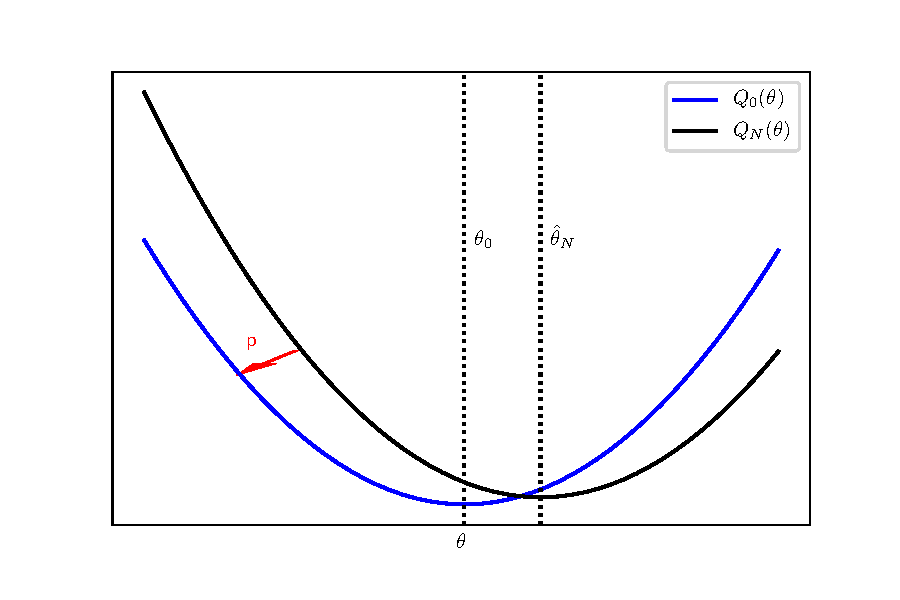
\includegraphics[width = \linewidth]{figures/extremumconv}
\caption*{As $N$ increases consistency will mean for the criterion function $Q_N(\theta)$ to converge in probability to the actual criterion function $Q_0(\theta)$, thus yielding a consistent estimate of $\hat{\theta}_N$.}
\end{figure}

We can think of $Q_N(\cdot)$ as the sample criterion function, which when minimized yields a sample parameter estimate $\hat{\theta}_0$, and likelise the population criterion $Q_0(\cdot)$ yields the true parameter $\theta_0$. The goal in showing consistency is to show that the sample criterion converges in probability to $Q_0(\cdot)$. For M-estimators applying a law of large numbers gives that
\begin{equation}
\frac{1}{N} \sum_{i=1}^N q(w_i, \theta) \underset{N \rightarrow \infty}{\rightarrow} E[q(w_i, \theta)] \equiv Q_0(\theta)
\end{equation}
but this is not possible in the case of extremum estimators. Instead, c.f theorem 5.1 of C\&T the following assumptions will ensure that an estimator $\hat{\theta}_N$ is consistent:
\begin{itemize}
\item The parameter space $\Theta$ is a compact subset of $\mathbb{R}^q$, compact meaning closed an bounded. (Note that $\mathbb{R}$ is not compact, making this asusmptions untrue for most estimation methods in practise).
\item $Q_N(\theta)$ is measurable and continous for all $\theta \in \Theta$.
\item $Q_N(\theta)$ converges uniformly in probability to a nonstochastic function $Q_0(\theta)$, which has a unique global maximum at $\theta_0$.
\end{itemize}
Assuming continuity and measurability of $Q_N(\theta)$ and compactness of $\Theta$ allows to invoke the extreme value theorem, which simply guarantees that a minimum and amaximum of $Q_N(\cdot)$ over a closed interval $[a,b]$ will exist.

\subsection{Asymptotic distribution}
To derive the limit distribution of $\hat{\theta}_N$ we will invoke the \textit{mean value theorem}, which has a very intuitive graphical presentation shown in figure \ref{fig: MVT}. Mathematically we simply equate the derivative of a function, measured in a point $x^+$ with the slope of a line connecting two points $[x_0,x_1]$. To use the theorem it is required that $Q_N(\cdot)$ is twice differentiable around $\theta_0$. Applying the mean value theorem on $\frac{\partial Q_N(\theta)}{\partial \theta}$ on the interval $[\hat{\theta}_N, \theta_0]$ will yield

\begin{multline}
\frac{\partial Q_N(\theta)}{\partial \theta} \bigg{|}_{\hat{\theta}_N} =
\frac{\partial Q_N(\theta)}{\partial \theta} \bigg{|}_{\theta_0} \\ +
\frac{\partial^2 Q_N(\theta)}{\partial \theta \partial \theta'} \bigg{|}_{\theta^+}(\hat{\theta}_N - \theta_0)
\end{multline}

Where by definition $\frac{\partial Q_N(\theta)}{\partial \theta} \bigg{|}_{\hat{\theta}_N} = 0$ so rearranging leaves us with


\begin{multline} \label{eq: asyms}
\sqrt{N}(\hat{\theta}_N - \theta_0) = \left( \frac{\partial^2 Q_N(\theta)}{\partial \theta \partial \theta'} \bigg{|}_{\theta^+} \right)^{-1}  \\ \times
\left(
\frac{\partial Q_N(\theta)}{\partial \theta} \bigg{|}_{\theta_0} \sqrt{N}
\right)
\end{multline}


\begin{figure}
\caption{Mean Value Theorem illustration}
\label{fig: MVT}
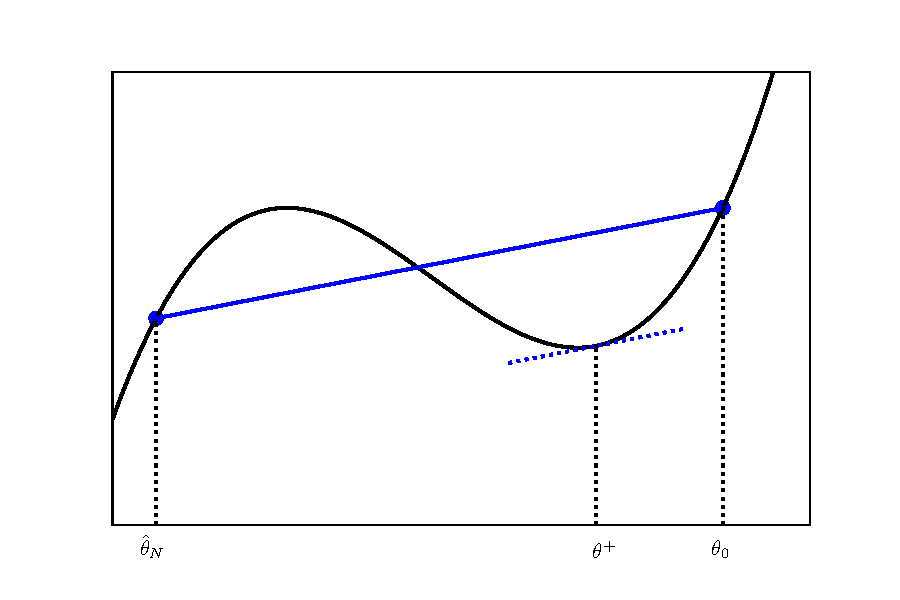
\includegraphics[width = \linewidth]{figures/mvt}
\caption*{The mean value theorem essentially tells us that any continous function $f(z)$ over the interval $\mathcal{I}$ will have at least one point in $\mathcal{I}$ where $\frac{\partial f(z)}{\partial z}$ equals the slope between the endpoints of $\mathcal{I}$.}
\end{figure}

It is then assumed that the following matrices exist and, that the terms converge towards
\begin{align*}
&\frac{\partial^2 Q_N(\theta)}{\partial \theta \partial \theta'} \bigg{|}_{\theta^+} \overset{p}{\rightarrow} A_0 \\
& \frac{\partial Q_N(\theta)}{\partial \theta} \bigg{|}_{\theta_0} \sqrt{N} \overset{d}{\rightarrow} \mathcal{N}(0,B_0)
\end{align*}
If $A_0$ and $B_0$ exist, we can then see from the expression in \eqref{eq: asyms} that asymptotically a consistent M estimator $\hat{\theta}_N$ has distribution
 \begin{equation}
 \sqrt{N}(\hat{\theta}_N - \theta_0) \overset{d}{\rightarrow} \mathcal{N}(0, A_0^{-1}B_0A_0^{-1})
 \end{equation}
In practise of course $A_0$ and $B_0$ are unknown, and will have to be estimated, usually with the following empirical matrices

\begin{align*}
&\hat{A} = \frac{\partial^2 Q_N(\theta)}{\partial \theta \partial \theta'} \bigg{|}_{\hat{\theta}}
\\
& \hat{B} = \frac{1}{N} \sum_{i=1}^N \frac{\partial q(w_i, \theta)}{\partial \theta} \bigg{|}_{\hat{\theta}} \frac{\partial q(w_i, \theta)}{\partial \theta'} \bigg{|}_{\hat{\theta}}
\end{align*}

\subsubsection{Maximum likelihood estimators}
Maximum likelihood estimators has the property that $Q_N(\theta)$ is specified so that
\begin{equation}
Q_N(\theta) = - \sum_{i=1}^N \log L_i(\theta| x_i,y_i)
\end{equation}
Because of this the sandwich expression for the variance derived above collapses to an even simpler expression where $\hat{\theta}_{ML} \sim \mathcal{N}(0, [\mathcal{I}(\theta)]^{-1})$ where $\mathcal{I}(\theta)$ is the fischer information, defined as
\begin{equation}
\mathcal{I}(\theta) = -E\left[ \frac{\partial^2 \log L_i(\theta| x_i,y_i)}{\partial \theta \partial \theta'} \right]
\end{equation}
The proof of this is as follows

Use that $\log L_i(\theta |x_i, y_i) \propto f(y_i | \theta)$, that is the likelihood is proportional to the density of the data. Starting here, we know that
\begin{equation}
\int_{\mathbb{R}} f(y_i | \theta) = 1
\end{equation}
and since the bound of the integral does not depend on $\theta$ taking the derivative w.r.t it on both sides gives
\begin{equation}
\int_{\mathbb{R}} \frac{\partial}{\partial \theta} f(y_i | \theta) = 0
\end{equation}
Now apply that $\frac{\partial \log f(x)}{\partial x} = \frac{\partial f(x)}{\partial x} [f(x)]^{-1}$ to get
\begin{equation}
\int_{\mathbb{R}} \frac{\partial \log f(y_i | \theta)}{\partial \theta}  f(y_i | \theta) = 0
\end{equation}
Using again the rewrite of the derivative of the log of a function gives
\begin{align}
&\int_{\mathbb{R}} \frac{\partial}{\partial \theta} \frac{\partial \log f(y_i | \theta)}{\partial \theta}  f(y_i | \theta) = 0
\end{align}
Which when written out gives
\begin{align*}
 \int_{\mathbb{R}}  &\frac{\partial \log f(y_i | \theta)}{\partial \theta}  \frac{\partial f(y_i | \theta)}{\partial \theta}
\\ &+ \frac{\partial^2 \log f(y_i | \theta)}{\partial \theta \partial \theta'} f(y_i|\theta)
 = 0
\end{align*}
Using the log-derivative trick one final time gives the desired result
\begin{align*}
 \int_{\mathbb{R}}  &\frac{\partial f(y_i | \theta)}{\partial \theta}  \frac{\partial f(y_i | \theta)}{\partial \theta} f(y_i | \theta)
\\ &+ \frac{\partial^2 \log f(y_i | \theta)}{\partial \theta \partial \theta'} f(y_i|\theta)
 = 0
\end{align*}
Or written in terms of expectations
\begin{equation}
E \left[
\frac{\partial f(y_i | \theta)}{\partial \theta}  \frac{\partial f(y_i | \theta)}{\partial \theta}
\right]
= - E\left[
\frac{\partial^2 \log f(y_i | \theta)}{\partial \theta \partial \theta'}
\right]
\end{equation}
Comparing this expression to the $A_0^{-1}B_0A_0^{-1}$ expression derived above should make it clear why the asymptotic variance of maximum likelihood estimators simplifies to the fischer information.


\section{Numerical optimization}
The motivation behind numerical optimization is simple: often we come across functions that are difficult to optimize analytically, and in any case computers are not very good at analytical math. Instead of solving problems exactly, we would like to have methods which come close to the true solution without being to computationally intensive.

In the lectures a host of topics including steepest descent optimization and non-gradient based methods were covered, but here we'll only give a brief overview of the Newton Rhapson algorithm.

\subsection{The Newton Rhapson algorithm}
The idea of the Newton Rhapson algorithm is to intiate the maximization of a function $f(x)$ at some starting guess $x_0$, where a second order Taylor polynomial $p(x_0)$ is constructed. The next point in the procedure will then be the $x=x^1$ where $p(x_1)$ is minimized. The algorithm is generalized to the multivariate case, but the intuition nonetheless remains the same. Let $x_o \in \mathbb{R}^p$ then the second order Taylor approximation of $f(\cdot)$ around $x_0$ is
\begin{multline}
p(x) = f(x_0) + \nabla f(x_0) (x- x_0) \\+ (x-x_0)'\frac{\nabla^2 f(x_0)}{2}(x-x_0)
\end{multline}
for which there is naturally only one solution when solving $p'(x) = 0$, which is the one where
\begin{equation}
x = x_0 - [\nabla^2 f(x_0)]^{-1} \nabla f(x_0)
\end{equation}
This equation gives the next point $x$ to approximate as a function of the current point of approximation $x_0$. It should be noted that the second term is essentially \textit{slope over curvature}. Generalizing the above equation to an iterative algorithm leads to the Newton Rhapson equation
\begin{equation}
x_{n+1} = x_n - s_n [\nabla^2 f(x_n)]^{-1} \nabla f(x_n)
\end{equation}
where $s_n$ is some arbitrarily chosen step size, which ensures the algorithm doesn't get stuck in a steady state, where it jumps back and forth between two suboptimal points.

\subsubsection{Berndt-Hall-Hall-Hausman (BHHH)}
Computationally estimating the hessian at every step might be to costly, so as an alternative the BHHH algorithm utilizes the results derived for ML estimators above, and estimates the hessian as a product of gradients, that is
\begin{equation}
\frac{\partial^2 Q_N(x)}{\partial x \partial x'} \approx \sum_{i=1}^N \frac{\partial q_i(x)}{\partial x} \frac{\partial q_i(x)}{\partial x'}
\end{equation}
with this procedure it is only neccesary to estimate the gradient, which is much less costly than computing the hessian. On the other hand, if the model is wrongly specified, or the sample is small BHHH will perform poorly.


\section{Nonlinear least squares}
Nonlinear least squares is, as the name suggests similar to OLS, but with the added ability to handle nonlinear relations. Before jumping to use NLS, it should however be considered if the relationship of interest is nonlinear even when considering variable transformations. If this not is the case, NLS might be the right choice of estimator. We begin by defining the model, noting that NLS is a M-estimator, due to the form of it's criterion function.

\begin{equation}
y_i = g(x_i, \beta) + u_i, \qquad E[y_i | x_i] = g(x_i, \beta)
\end{equation}
This is very similiar to OLS, but with the addition of a link function $g(\cdot)$, which alters the estimation problem to
\begin{equation}
\hat{\beta}_{NLS} = \underset{\beta}{\textrm{arg max }} \sum_{i=1}^N (y_i - g(x_i, \beta))^2
\end{equation}
Taking the first order conditions is straight forward from here, simply solve $\frac{\partial Q_N(\beta)}{\partial \beta} = 0$. Results on the asymptotic distribution of $\hat{\beta}_{NLS}$ follows from theory on M-estimators.

It can be shown that NLS will be consistent, but not nessecarily efficient if $E[u_i | x_i]=0$, as this assumption alone doesn't account for heteroscedasticity. To account for this, the idea is to implement a weight in the optimization problem. We can show that the optimal weight is the actual variance-covariance matrix $\Omega_0$
\begin{equation}
V[y_i | x_i] = V[u_i|x_i] = E[uu'|x] = \Omega_0
\end{equation}
Of course $\Omega_0$ is unknown, so instead of using this, we begin by simply guessing a matrix $\Sigma$ and estimating $\hat{\beta}_{WNLS}$ as
\begin{equation}
\underset{\beta}{\textrm{arg min }} (y-g(x,\beta))'\Sigma^{-1}(y-g(x,\beta))
\end{equation}
One way to select $\Sigma$ is then to assume that it depends on a set of parameters $\gamma$ and estimate $\hat{\Sigma}=\Sigma(\hat{\gamma})$. In practise this is implemented in steps
\begin{itemize}
\item[1.] Do regular NLS to estimate $\hat{\beta}_{NLS}$
\item[2.] compute the residuals $\hat{u}_i = y_i - g(x_i, \hat{\beta}_{NLS})$ and regress their square on a guessed variance matrix structure and covariates $\gamma$ to get $\hat{\Sigma}$.
\item[3.] Implement the estimated $\hat{\Sigma}$ and conpute the WNLS estimator.
\end{itemize}
This procedure can theoretically be iterated over multiple times, each time refining the estimate of $\hat{\gamma}$ and thus of $\hat{\Sigma}$.



\section{Binary response models - probit and logit}
Binary response models are designed to be useful whenever the outcome of interest can take only one of two values, i.e. $y_i \in \{0,1\}$, where $y_i=0$ happens with probability $1-p_i$ and conversely $\textrm{Pr}(y_i = 1)=p_i$. To include observable characteristics we parametrize the probability by a linear relation of dependents and a link function $F(\cdot)$ such that
\begin{equation}
p_i \equiv \textrm{Pr}(y_i = 1 | x_i) = F(x_i'\beta)
\end{equation}
Since $F(\cdot)$ must be confined in the interval $[0,1]$ and represents a probability, we will usually select $F(\cdot)$ to be a CDF. Common choices are the logistic CDF $\Lambda(\cdot)$ and the normal CDF $\Phi(\cdot)$.

\begin{align*}
\Lambda(z) &= \frac{\exp(z)}{1 + \exp{z}} \\
\Phi(z) &= \int_{-\infty}^{z} \phi(w) \textrm{d}w
\end{align*}
with $\phi(\cdot)$ begin the density of a gausian variable with mean 0 and variance 1.

\subsection{Maximum Likelihood estimation}
Notice that conditional on $x_i$ the outcome of $y_i$ is essentially a bernoulli trial, so the density of $y_i$ will be
\begin{equation}
f(y_i|\theta) = p_i^{y_i}(1-p_i)^{1-y_i}
\end{equation}
Inserting the link function and assuming independence of observations allow us to construct a full sample likelihood given by
\begin{equation*}
L_N(\theta) = \prod_{i=1}^N   F(x_i' \beta)^{y_i}(1-F(x_i'\beta))^{1-y_i}
\end{equation*}
The log likelihood function is then easily derived by taking the log, which transforms the product into a sum, draws down the exponents,
\begin{equation}
\mathcal{L}(\theta) = \sum_{i=1}^N \log L_i(\theta|x_i, y_i)
\end{equation}
From here it's possible to derive the scores $s_N(\theta)$ by taking the first derivative, and with a lot of work the hessian is also analytically derivable. The equation system $s_N(\theta)=0$ is however not analytically solveable but requires numerical methods.

\subsection{Latent variable representation}
An alternative to the derivations above is to assume the existence of a latent, unobservable variable. This variable $y^*$ acts as an underlying continous variable, which indirectly determines $y$ through a cutoff value, that is
\begin{equation}
y_i = \begin{cases}
1, \quad y_i^* > 0 \\
0, \quad y_i^* \leq 0
\end{cases}
\end{equation}
Where we assume $y_i*$ to be linear, i.e.
\begin{equation}
y_i^* = x_i' \beta + \epsilon_i
\end{equation}
The interpretation of $y_i^*$ can be as a utility variable, where individuals gaining more than $y_i^* = 0$ utility will make a certain choice, which we record as $y_i = 1$. Now instead of assuming a certain link function, we will make a distributional assumption on the error term $\epsilon_i$. In the following we assume that $\epsilon_i \sim \mathcal{N}(\mu, \sigma^2)$ to derive the probit model. First of calculate the probability of observing $y_i = 1$
\begin{align*}
p_i \equiv \textrm{P}(y_i = 1| x_i) &= \textrm{P}(y_i^* > 0 | x_i) \\
& = \textrm(P)(x_i'\beta + \epsilon_i > 0 | x_i)
\\
& = 1-\textrm{P}(\epsilon_i \leq -x_i'\beta | x_i)
\end{align*}
To finalize this we first need to normalize $\epsilon_i$ to be drawn from a standard normal distribution
\begin{align*}
p_i&=1-\textrm{P}\left(\frac{\epsilon_i - \mu}{\sigma} \leq  -\frac{x_i'\beta + \mu}{\sigma} | x_i \right)
\end{align*}
Which then is rewriteable into the final expression, by using that $\epsilon_i$ is normally distributed, and that this distribution is symmetric meaning $1-\Phi(-z)=\Phi(z)$
\begin{equation}
p_i = \Phi\left(\frac{x_i'\beta + \mu}{\sigma} \right)
\end{equation}
This $p_i$ is the same one defined and parametrized as $F(\cdot)$ in the non-latent interpretation, showing us that whether we choose a latent-variable aproach to the model or not, we end up with the same conclusions. From the expression of $p_i$ it's clear that neither $\beta$ or $\mu$ are going to be present on their own in the likelihood function, as they are always divided by $\sigma$. Thus identification requires fixing $\sigma$. Usually we set $\sigma = 1$ to get the simplest expression of $\beta$'s $\Phi(x_i'\beta + \mu)$ with $\mu=0$ usually also implemented as the intercept of the model is otherwise not identified. The logit model has a natural scale of $\mu=0$ and $\sigma^2 = \pi^2/3$, so results between the two models are not directly comparable.

\subsection{Marginal effects}
The regression coefficients in the probit and logit model are uninformative as they depend on the scale of errors, and are not in any simple way related to the observed $y_i$'s. Instead one may study the marginal effects of changing a covariate $x_{ij}$ on the probability that $y=1$, that is
\begin{equation}
  \frac{\partial \textrm{Pr}(y_i = 1 | x_i)}{\partial x_{ij}} = F'(x_i'\beta)\beta_j
\end{equation}
Often this partial derivative is denoted $\delta_j(x_i)$. In the case of dummy variables, $\delta_j$ is simply calculated as the difference in probability with the dummy on and off, keeping all other covariates constant. Marginal effects depend nonlinearly on $x_i$, and thus change depending on the observation for which they are calculated. In practise there are a number of ways to handle this. Some researchers choose a specific individual $i$ (i.e. the median individual) and compute marginal effects only for this observation, or for the 'mean' individual where $\bar{x}=\frac{1}{N}\sum_{i}x_i$ is used as covariates. Others compute marginal effects for all observations and report their average.

\subsubsection{The Delta method}
One issue with the marginal effects derived above is that while they depend on $\beta$, and so in practice also on $\hat{\beta}$, we cannot derive an expression for their standard errors. To get an estimate of these one option is the Delta method, which in general derives approximate standard errors for function of variables with known errors. An alternative approach is to bootstrap sample from the dataset, which is covered later in this note. In the most general case the delta method can be used to show that
\begin{equation}
  V[h(\hat{\beta})] \approx \frac{\partial h(\hat{\beta})}{\partial \beta'}V[\hat{\beta}]\frac{\partial h(\hat{\beta})}{\partial \beta}
\end{equation}
where $h(\cdot)$ is any function of $\beta$.

In the case of the probit model begin by noting that the the marginal effects are rewriteable as
\begin{equation}
\delta_k(x_i) = F'(x_i'\beta)|_{x_i = x^0}\beta_k = g(x^0\beta)\beta_k
\end{equation}
where $g(\cdot)$ is simply shorthand for $F'$ evaluated in $x^0$. $\delta_k$ is a function of parameters which we will denote $d_k(\beta)$ and the estimates partial effects are $\hat{\delta}_k = d_k(\hat{\beta})$. Stacking these in a column vector $\textbf{d}(\hat{\beta})$ gives is a $K\times 1$ column, for which we can do the following Taylor expansion around $\beta$
\begin{equation}
  \textbf{d}(\hat{\beta}) \approx \textbf{d}(\beta) + \nabla_{\beta}   \textbf{d}(\beta)(\beta - \hat{\beta})
\end{equation}
Rewriting that $\textbf{d}(\hat{\beta}) = \hat{\delta}$ we get that
\begin{equation}
  \hat{\delta} - \delta \approx \nabla_{\beta}   \textbf{d}(\beta)(\beta - \hat{\beta})
\end{equation}
Multiplying by $\sqrt{N}$ on both sides, and noting that $\hat{\beta}\sim \mathcal{N}(0,V[\beta])$ we get that
\begin{equation}
  \hat{\delta} \overset{a}{\sim} \mathcal{N}(0, [\nabla_{\beta}   \textbf{d}(\beta)]V[\beta][\nabla_{\beta}   \textbf{d}(\beta)]')
\end{equation}
Now we dont know $\nabla_{\beta} \textbf{d}(\beta)$ yet, but it is easily derived. Use the definition of $\delta_k$ from above and we have that
\begin{align*}
  \nabla_{\beta} \textbf{d}(\beta) &= \frac{\partial}{\partial \beta} g(x^0\beta) \beta \\
  & = \beta \frac{\partial}{\partial \beta} \left[
g(x_0\beta)
  \right] +
I_k  g(x^0\beta) \\
  &= \beta g'(x^0\beta)x^0 + I_k g(x^0)
\end{align*}
where $I_k$ is the identity matrix. This is as far as we can get without further assumptions, but in the probit case we can utilize that $g(\cdot)$ is the normal pdf $\phi(\cdot)$, for which it holds that $\phi'(z)=-z\phi(z)$\footnote{\textbf{Proof}: let $\phi(z)=(2\pi)^{-1/2}\exp(\frac{-z^2}{2} )$, then by differentiating $\phi'(z)= (2\pi)^{-1/2}\exp(\frac{-z^2}{2})\cdot \left(\frac{-2}{2}\cdot z \right)$ which clearly reduces to $\phi'(z)=-z\phi(z)$}. When this is the case simply inserting $\phi'(x^0\beta)=-(x^0\beta)'\phi(x^0\beta)'$ and factoring out will give the desired result shown in the lecture.


\section{Censored regression models}
The Tobit model is designed to handle data with unnatural cutoffs, either due to censoring or traits of the DGP. An important distinction to make is between \textit{censoring}, which keeps all observations, but censors certain of them to an arbitrary value and \textit{truncation} which remove all observations at or below a certain threshold from the dataset. The Tobit model is formulated in terms of a latent variable $y^*$, so to begin with let
\begin{equation}
y_i^* = x_i'\beta + \epsilon_i, \quad \epsilon_i \sim \mathcal{N}(0, \sigma^2)
\end{equation}
The observational rule is slightly modified compared to the binary case, as we now have $y_i = \max\{0, y_i^*\}$.

\subsection{Maximum Likelihood estimation}
In the case of the Tobit model the likelihood is multiplicatively separable into the likelihood from observations where $y_i=0$ and the likelihood from observations where $y_i >0$, that is
\begin{equation}
  f(y_i|x_i) =
   \begin{cases}
     f_0(y_i|x_i), \quad \textrm{if }y_i = 0 \\
     f_1(y_i|x_i), \quad \textrm{if }y_i > 0
   \end{cases}
\end{equation}
Which, as will later come in handy, can be condensed to a product of factors raised to indicators for the case. In the face of $f_0(\cdot)$ this is equal to the probability that $y_i=0$. Following the same steps as in the probit example, inserting $y^*_i$ and isolating $\epsilon_i$ will provide that
\begin{equation}
  f_0(y_i|x_i) = 1 - \Phi \left(\frac{x_i'\beta}{\sigma}\right)
\end{equation}
On the other hand when $y_i>0$ we know that we're observing the actual latent variable $y^*$, and from the definition of this variable it's clear that $y^*_i|x_i \sim \mathcal{N}(x_i'\beta, \sigma^2)$. Thus\footnote{the expression of $f_1$ is simply a clever way to write a non-standard normal distribution without having to write the entire pdf. Be aware that $\phi(z)$ is always the pdf of a standard normal.}
\begin{equation}
  f_1(y_i|x_i) = \frac{1}{\sigma} \phi\left( \frac{y_i - x_i'\beta}{\sigma}
  \right)
\end{equation}
Now these expression can be joined as follows
\begin{multline}
f(y_i| x_i) =
\left[
1 - \Phi \left(\frac{x_i'\beta}{\sigma}\right)
\right]^{\mathds{1}_{(y_i = 0)}}  \\
\times
\left[\frac{1}{\sigma} \phi\left( \frac{y_i - x_i'\beta}{\sigma}
\right)\right]^{\mathds{1}_{y_i > 0}}
\end{multline}
The indvidual (log) likelihood contributions as well as the overall (log) likelihood function are then easy to derive. The score is difficult to find, and the first order condition has no analytical solution, so numerical methods must be used. Notice there are a number of ways to answer questions about the expected value of our model, specifically we might be interested in $E[y^*|x]$, $E[y|x]$ or $E[y| y>0, x]$. The first one is simple, $E[y^*|x]= x'\beta$, but the other two are slightly less straight forward. In all cases the same method is applied, namely substituting in $y^* = x'\beta + \epsilon$ and isolating stochastic terms. For example
\begin{equation}
\begin{split}
E[y| y>0, x] &= E[x'\beta + \epsilon |x'\beta + \epsilon > 0 , x] \\
& = x'\beta + E[\epsilon| \epsilon > -x'\beta, x] \\
& = x'\beta + \sigma E\left[\frac{\epsilon}{\sigma}| \frac{\epsilon}{\sigma}> \frac{x'\beta}{\sigma}, x\right] \\
& = x'\beta + \sigma \lambda \left(\frac{x'\beta}{\sigma}\right)
\end{split}
\end{equation}
Where a number of tricks are used. In line 3 we multiply and divide by $\sigma$ to get a standard normal in the expectation, and below in line 4 that for any $X\sim\mathcal{N}(\mu,\sigma)$ we have that the inverse Mills ratio $\lambda(z)$ is  $E[X|X>\alpha]=\frac{\phi(z)}{1- \Phi(z)}$ where $z = \frac{\alpha-\mu }{\sigma}$. To derive $E[y|x]$ first notice that this must be $\textrm{Pr}(y=0)\cdot 0 + \textrm{Pr}(y>0)\cdot E[y|y>0, x]$ and $\textrm{Pr}(y>0)$ is
\begin{equation}
\begin{split}
\textrm{Pr}(y>0) &= \textrm{Pr}(x'\beta + \epsilon>0) \\
& = \textrm{Pr}(\epsilon > - x'\beta) \\
& =1 - \textrm{Pr}\left(\frac{\epsilon}{\sigma} \leq \frac{-x'\beta}{\sigma}\right) \\
& = 1- \Phi \left(\frac{-x'\beta}{\sigma}\right) \\
& = \Phi \left(\frac{x'\beta}{\sigma}\right)
\end{split}
\end{equation}
Since $\lambda(z) \equiv \frac{\phi(z)}{\Phi(z)}$ is is then clear how
\begin{equation}
E[y|x] = x'\beta \Phi \left(\frac{x'\beta}{\sigma}\right) + \sigma \phi \left(\frac{x'\beta}{\sigma}\right)
\end{equation}

Marginal effects are ususally calculated on these quantities, and should be straight forward to derive, simply by calculating $\frac{\partial}{\partial x}$ in one of the above expectations or probabilities.



\section{Multinomial Logit models}
Multinomial choice models are models concerned with ordered or unordered choices, i.e. the choice of education, which car to buy or similar. The common trait of all problems which can be modelled by multinomial models is the discrete choice levels available. The following models are all concerned with unordered choices, (i.e. not education, which is a 'ladder-choice'). Our goal is to specify and estimate a utility function $u: (x_{ij}, \theta)\mapsto \mathbb{R}$ and estimate this mapping such that $\forall j, \theta' : u(x_{ij}, \theta)>u(x_{ij}, \theta')$. In the following we will study three variations of the model class \textit{Random Utility Models} (RAM), which is generally defined by the following construct of $u_i$
\begin{equation}
y_i = \underset{j \in \{1,2,...,J \} }{\textrm{arg max}} u_{ij}
\end{equation}
where $u_{ij}=v_{ij}+\epsilon{ij}$ consists of a deterministic/observable term $v$ and a stochastic/unobservable term $\epsilon$. The parametrization of $v$ will determine the type of RAM estimated amongst the conditional- (CL) multinnomial (MNL) and mixed logit models.
\begin{itemize}
\item[]\textbf{CL:}   \qquad     $v_{ij} =x_{ij}\beta $
\item[]\textbf{MNL:}    \quad   $v_{ij} = x_{i}\beta_j$
\item[]\textbf{Mixed:}  \  \  $v_{ij} = x_{ij}\beta + w_{i} \gamma_j $
\end{itemize}
In the conditional logit $x$ will contain information on the alternatives in $J$, while in the multinomial it will contain information on the individual $i$. To determine if all models are identified we need to first specify the likelihood function.

\subsection{Maximum Likelihood estimation}
Each individual makes only one choice, and so each individual will only contribute likelihood for this choice. To capture this idea define $d_{ij}=\mathds{1}_{(y_i = j)}$, which will be 1 for individual $i$ only if individual i made choice $j$, and 0 otherwise. To ensure that each individual cannot choose multiple values in $J$ we will require
\begin{equation}
\forall i: \sum_{j=1}^J d_{ij} = 1
\end{equation}
With this notation we can define the probability that $i$ chooses $j$ as
\begin{equation}
p_{ij}\equiv \textrm{Pr}(d_{ij}=1, d_{ik} = 0 \ \forall k\neq j)
\end{equation}
The individuals likelihood contribution will then be the product of these $p_{ij}$'s, but only counting the one for the exact value of $j$ what individual $i$ actually chose, so
\begin{equation}
\begin{split}
&\ell_i(\theta) = \prod_{j=1}^J p_{ij}^{d_{ij}} \\
& \log \ell(\theta) = \sum_{j=1}^J d_{ij} \log(p_{ij})
\end{split}
\end{equation}


\subsubsection{Specifying $p_{ij}$}
To finish we need an expression for $p_{ij}$, it can be shown that it's distribution will depend on the difference $\epsilon_{ij}-\epsilon_{ik}$ and further that assuming $\epsilon \sim \textrm{Gumbel}$ will result in the difference of two epsilons being logistically distributed. Thus we assume
\begin{equation}
\begin{split}
&F(\epsilon) = \exp(-\exp(-\epsilon)) \\
& f(\epsilon) = \exp(-\epsilon -\exp(-\epsilon))
\end{split}
\end{equation}
This assumption implies that
\begin{equation}
p_{ij} = \frac{\exp(v_{ij})}{ \sum_{k=1}^J \exp(v_{ik})}
\end{equation}
where $v_{ij}$ will vary depending on the model specification.
\\ \\
With this information we can complete the likelihood, by taking the product over the individual likelihood contributions, or equivalent in log-likelihood terms
\begin{equation*}
\log \mathcal{L}_N(\theta) = \sum_{i=1}^N \sum_{j=1}^J d_{ij} \log \left( \frac{\exp(v_{ij})}{ \sum_{k=1}^J \exp(v_{ik})}
\right)
\end{equation*}
By inserting the relevant specification of $v_{ij}$ and rewriting the log-term this expression simplifies slightly.

\subsection{Identification}
The derived expression of $p_{ij}$ implies specific requirements must be fulfilled to properly identify parameters in the model. What requirements exactly will depend on the specification of $v_{ij}$. In the conditional logit model adding an intercept $\beta_0$ to the model is problematic since
\begin{equation}
\frac{\beta_0 + \exp(v_{ij})}{ \sum_{k=1}^J  \exp(\beta_0 +v_{ik})} =
\frac{\exp(v_{ij})}{ \sum_{k=1}^J \exp(v_{ik})}
\end{equation}
so to identify the CL model the intercept needs to be fixed to 0. In the MNL model a constant $\delta$ can be added to $\beta_j$ in a similar fashion. The solution is then to fix the $\beta_j$ of one alternative as 1, making the specific alternative a baseline, against which other $\beta$'s should be compared. Naturally in the mixed model, both problems are present, and both restrictions need to be implemented.

\subsection{Marginal effects}
Marginal effects will depend on the model specification, beginning with the conditional logit, we have to consider two cases, namely that we take the derivative w.r.t the $x$ such that $j=k$ as well as the alaternative $j\neq k$. Beginning with the case of $j=k$ we calculate
\begin{equation}
\begin{split}
\frac{\partial \textrm{Pr}(y_i = j|x)}{\partial x_k} &= \frac{\partial}{\partial x_k} \frac{\exp(x_{ij}\beta )}{ \sum_{k=1}^J \exp(x_{ik}\beta)} \\
& = p_{ij}(1-p_{ik})\beta
\end{split}
\end{equation}
To get this result simply apply the derivative-of-a-fraction rule naively and compare the nominator and denominator in the resulting expression. You should be able to rewrite parts of the derivative as $p_{ik}$ and $p_{ij}$'s. The only tricky part is that although $j=k$ we need to keep the notation distinct to later accommodate the case where $j\neq k$. When this is the case the derivative changes slightly as the nominators derivative w.r.t $x_k$ is now 0, and there's an actual difference between differentiating w.r.t $x_k$ or $x_j$. Applying the derivate-of-a-fraction rule will now yield
\begin{equation}
\frac{\partial \textrm{Pr}(y_i = j|x)}{\partial x_k} = -p_{ij}p_{ik}\beta
\end{equation}
Combining these two expression is easily done with an indicator function, giving the final derivative
\begin{equation}
\frac{\partial \textrm{Pr}(y_i = j|x)}{\partial x_k}= p_{ij}(\mathds{1}_{(j=k)}-p_{ik})\beta
\end{equation}

In the case of the multinomial logit model the expression of $v_{ij}$ is different, and what's more important $x_{ij}$ is now constant across all alternatives $j$ so $x_{ij}=x_i$. Because of this, taking the derivative w.r.t some "$x_j$" is now meaningless, as there is no variation. A result is that as the sum in the denominator loops over $\beta_j$'s, each iteration will produce a non-0 result under differentiation. Again simply apply the same rule of differentiation to get the desired result, keeping in mind that $x$ is fixed across all alternatives, resulting in
\begin{equation}
\frac{\partial \textrm{Pr}(y_i = j|x)}{\partial x} = p_{ij}\left(
\beta_j - \sum_{l=1}^J p_{il}\beta_l
\right)
\end{equation}

Since the marginal effects are quite complicated and potentially non-linear, the log-odds ratio is often considered as an alternative. Defined simply as $\log(p_{ij}/p_{i1})$ where $p_{i1}$ is the probability of the baseline alternative, it is rather eqasy to show that this is equal to $x'_i \beta_j$ in the MNL case.

\subsubsection{Independence of irrelative alternatives}
A major drawback of the above models is that the relative probability of two choices $p_{ij}/p_{ik}$ does not depend on any other alternatives than $j$ and $k$, severely restricting how individuals can substitute between alternatives in this setup. 



\section{Quantile regression}
Quantiles are loosely for any given distribution the "$x$-values" matching up to a certain probability mass, covered by the distribution. In mathematical terms, with $\tau$ being some fraction of the total probability of 1, the quantile related to $\tau$ is $\mu_{\tau}$ which is given implicitly in
\begin{equation}
\tau = \textrm{Pr}(y \leq \mu_{\tau}) = F_{y}(\mu_{\tau})
\end{equation}
Normally $\mu_{\tau}$ is called the $\tau^{\textrm{th}}$ quantile, for example $\mu_{0.5}$ would be the $0.5^{\textrm{th}}$ quantile, or simply the median. Rewriting the above it's clear that $\mu_{\tau}=F^{-1}_y(\tau)$.
A parallel definition is that of conditional quantiles. These are simply taken to be conditional on some other variables $x$, for which the conditional distribution of $y$ is known, and possibly a set of parameters $\theta$, that is
\begin{equation}
\mu_{\tau}(x, \theta) = F^{-1}_{y|x}(\tau)
\end{equation}
How $F^{-1}(\cdot)$ is specified determines the amount of freedom in shaping the quantile lines. For example if $\mu(x, \beta_{\tau})=x' \beta_{\tau}$ each quantile must be linear, but can have a unique slope.

\subsection{Estimation}

\begin{figure}
\caption{$\rho$ function for quantile regression}
\label{fig: rhofunc}
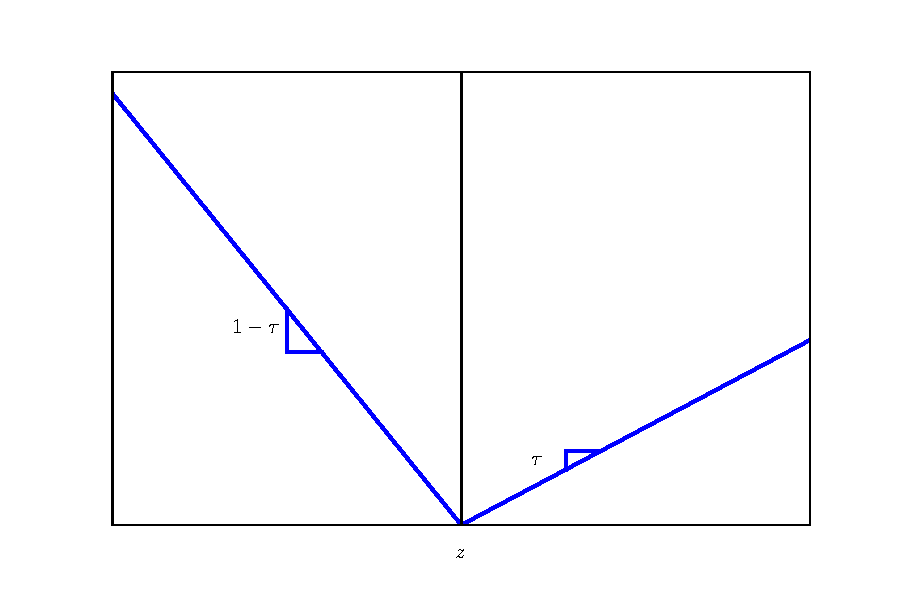
\includegraphics[width = \linewidth]{figures/rho}
\caption*{Notice how $\rho$ "weights" observations on either side of $z=0$ differently. This weighting ensures the propper result from the optimization problem.}
\end{figure}

Quantiles can also be defined as solutions to a minimization problem, specifically by defining $\rho(\cdot)$ as
\begin{equation}
\rho(z) = (\tau - \mathds{1}_{z<0}) \cdot z
\end{equation}
minimizing the expectation of $\rho(y_i - \mu_{\tau})$ will produce the $\tau^{\textrm{th}}$ quantile. Empirically we replace the expectation with a sum, and thus end up with the following estimator for $\hat{\mu}_{\tau}$
\begin{equation}
\hat{\mu}_{\tau} = \underset{\mu_{\tau} \in \mathbb{R}}{\textrm{arg min }} \sum_{i = 1}^N \rho(y_i - \mu_{\tau})
\end{equation}
Of course we're generally not interested in estimating constants. The mosst commonly used approach is to estimate conditional quantiles, whereby the value of $\mu$ depends on $x$ and parameters $\theta$, which are then the goal of optimization. In other words one normally solves
\begin{equation}
\hat{\theta}_{\tau} = \underset{\theta_{\tau} \in \mathbb{R}}{\textrm{arg min }} \sum_{i = 1}^N \rho(y_i - \mu(x_i, \theta_{\tau}))
\end{equation}
The lecture slides covers a heteroscedasticity model, as well as an example of quantile regression applied to birth weight. These are left out here. 


\section{Non- and semiparametric estimation methods}
As the name suggest non- and semiparametric estimation is a branch of econometrics concerned with estimating curves, densities etc. without assuming parametric functions for the relationships. Common for the nonarametric methods covered is that they essentially all are based off of generalizations of discrete counting estimators either in the form of histograms or binned scatterplots.

\subsection{Kernel Density estimators}
Begin by observing that a histogram can be constructed by counting the number of observations within a fixed distance from each $x_0$, so we can mathematically describe the value of a histogram at $x_0$ as
\begin{equation}
  \begin{split}
  \hat{f}_{\textsf{hist}}(x_0) &= \frac{1}{N} \sum_{i=1}^N \frac{\mathds{1}_{(x_0 - h \leq x_i \leq x_0 + h)}}{2h} \\
  & = \frac{1}{N\cdot h} \sum_{i=1}^N \mathds{1}_{\left(-1 \leq \frac{x_i - x_0}{h} \leq 1 \right)}
\end{split}
\end{equation}
where $2h$ (later respecified simply as $h$) is the bandwidth, i.e. the left-right distance from $x_0$ within which we count each $x_i$. The reason we divide with $2h$ and not just $h$ is that we count within a distance of $h$ on both the left and right side of $x_0$. Generalizing this to a kernel density estimator (KDE) is then as simple as moving from counting observations with the $\mathds{1}$-function, to computing a weighted sum using a kernel $K(z)$, thus in general we have
\begin{equation}
  \hat{f}(x_0) = \frac{1}{Nh} \sum_{i=1}^N K\left( \frac{x_i - x_0}{h} \right)
\end{equation}
where $K(z)$
\begin{itemize}
  \item[A)] Is continuous and symmetric around 0, i.e. $K(z)=K(-z)$.
  \item[B)] Integrates to one: $\int K(z) \textrm{d}z = 1$ and is mean zero: $\int z K(z) \textrm{d}z= 0$ (this is already given by the symmetry requirement).
  \item[C)] Is at least convergent to 0, for $|z|\rightarrow \infty$.
  \item[D)] Has non-infinite variance and constant, $\int z^2 K(z)\textrm{d}z = \kappa$, where $\kappa$ is some constant in $\mathbb{R}$.
\end{itemize}
The choice of kernel is not trivial, and several options exist. Often a regular gaussian distribution is used, but this has the disadvantage of assigning non-zero weight to all observations, meaning computations increase drastically with the number of observations. As alternatives triangle, uniform or Epanechnikov kernels might be used.

\subsubsection{Bias of the KDE estimator}


\end{document}
